\documentclass[a4paper]{book}
\usepackage[utf8]{inputenc}
\usepackage{graphicx}
\usepackage{amsfonts}
\usepackage{amsmath}
\usepackage{amssymb}
\usepackage{titling}
\usepackage{hyperref}
\usepackage{xcolor}
\usepackage{pagecolor}
\usepackage{eso-pic}

\newcommand\BackgroundPic{%
	\put(0,0){%
		\parbox[b][\paperheight]{\paperwidth}{%
			\vfill
			\centering
			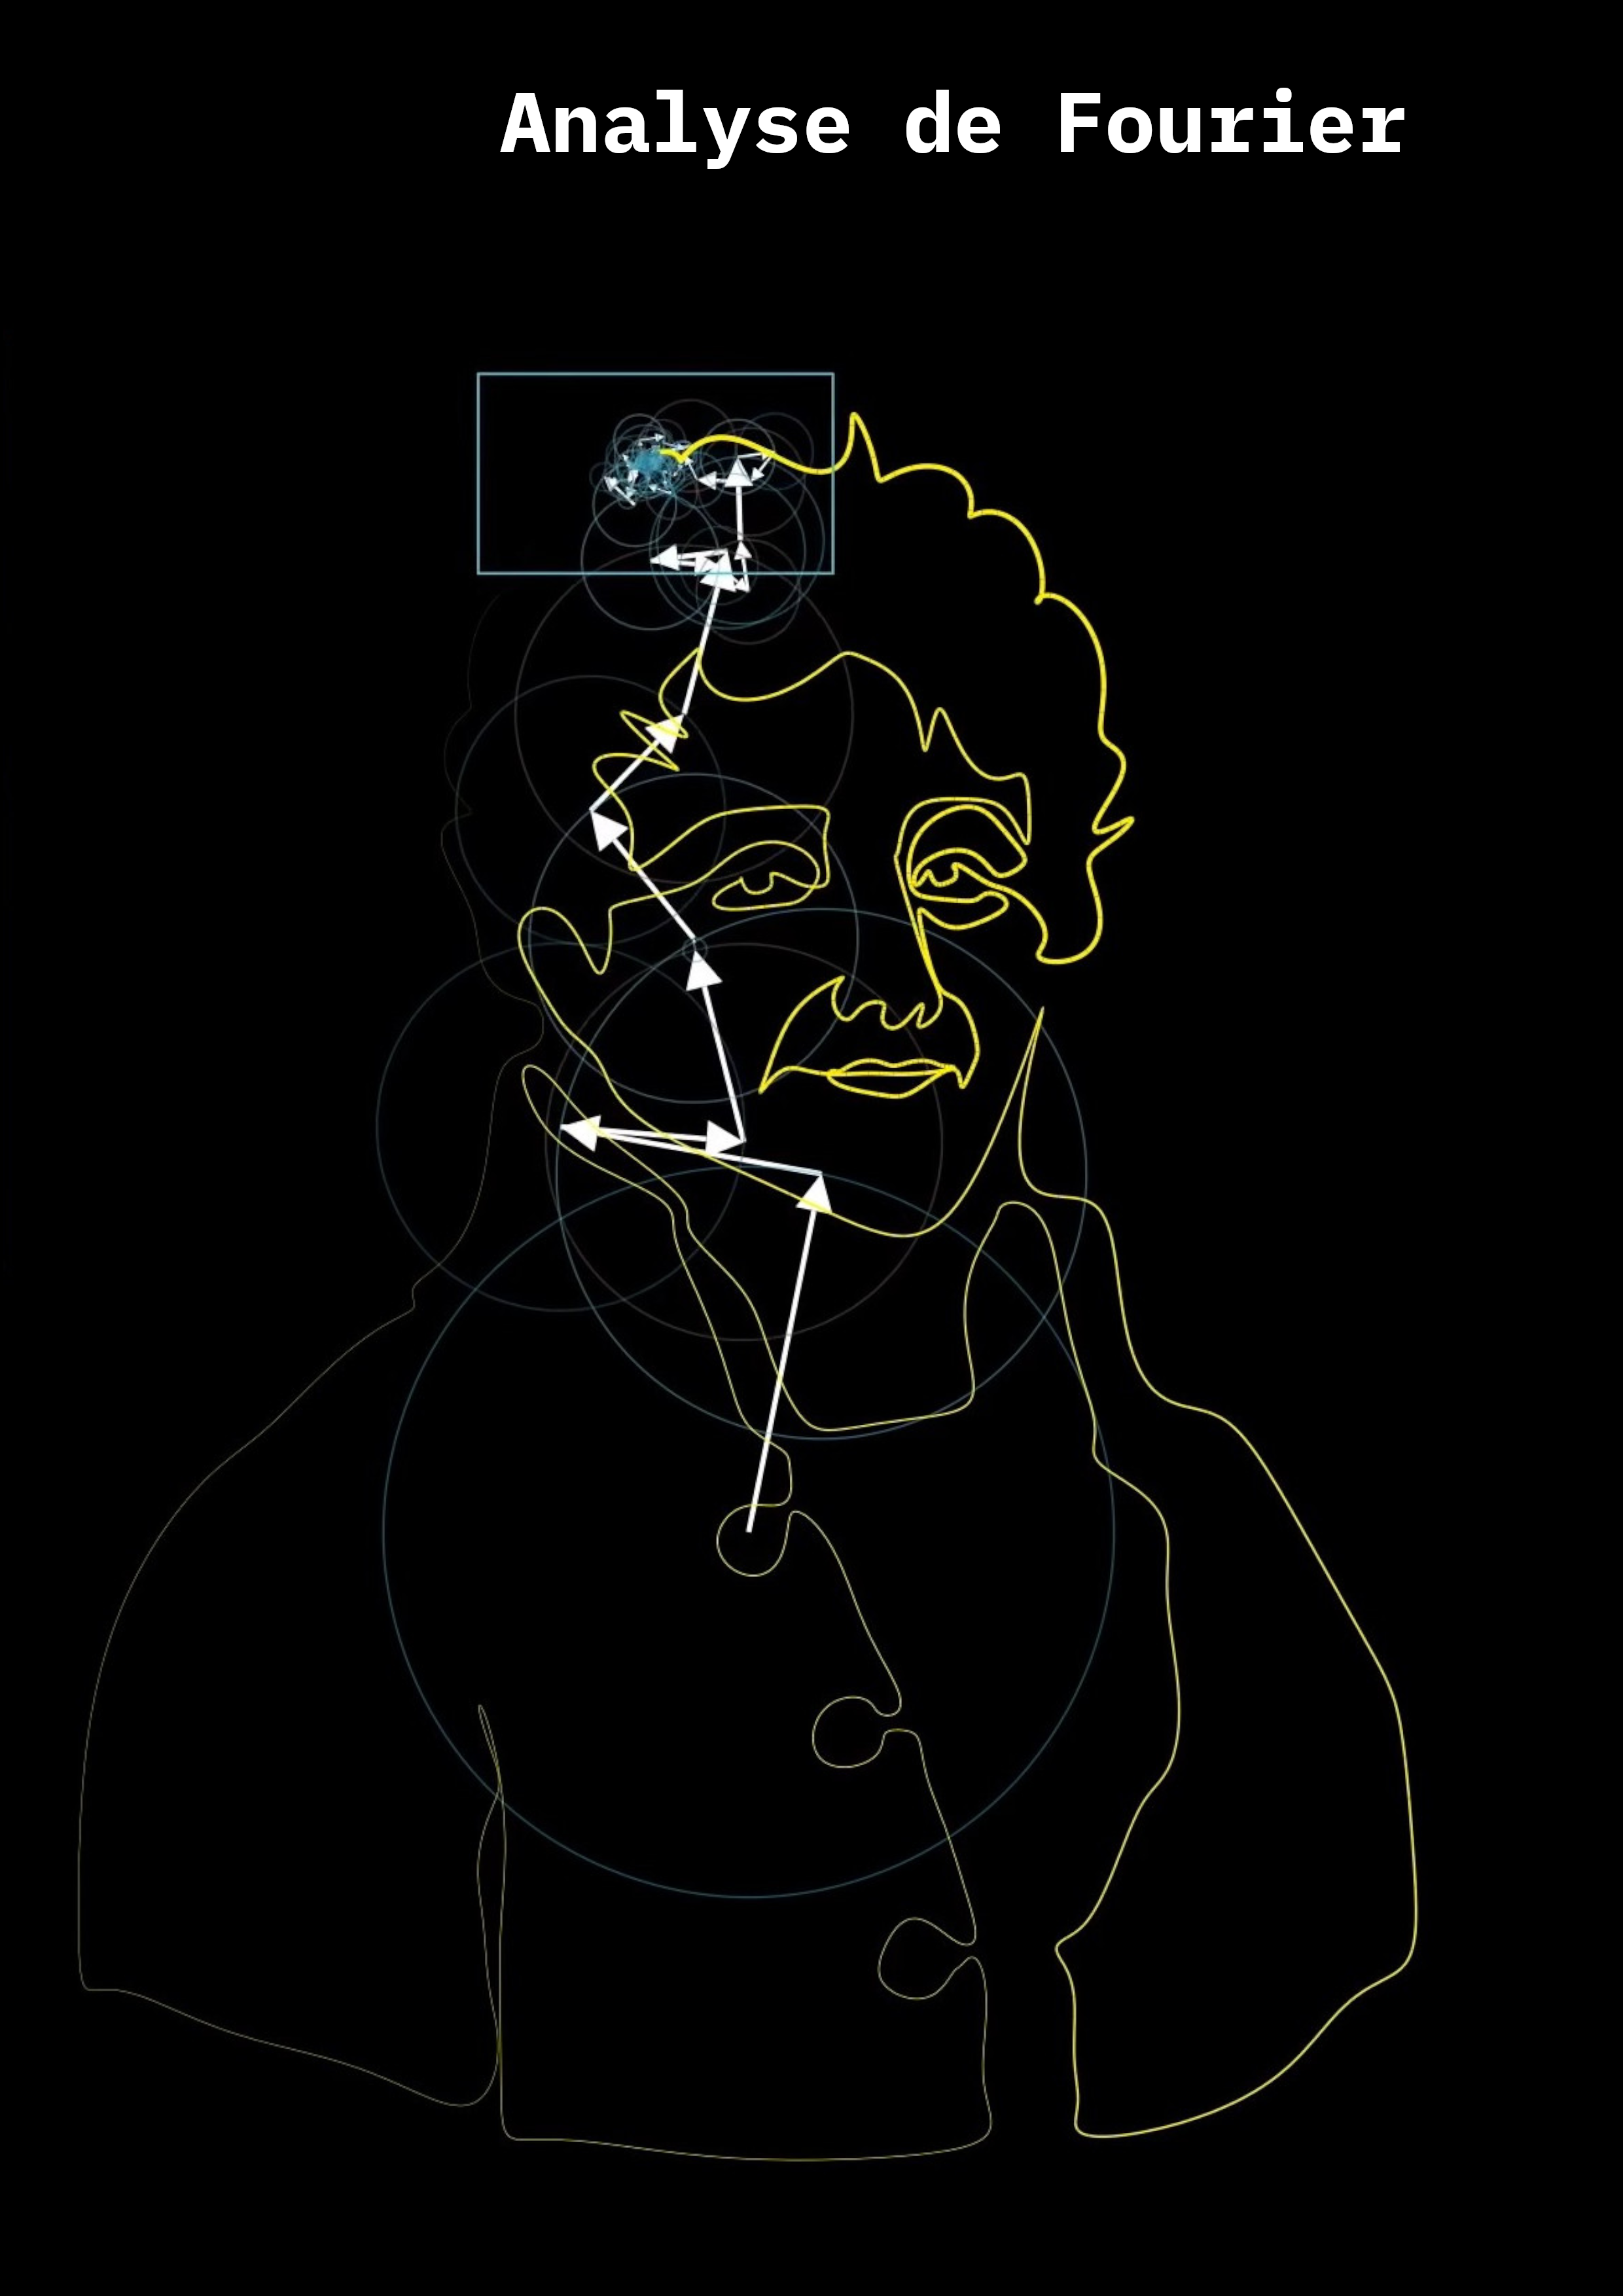
\includegraphics[width=\paperwidth,height=\paperheight,%
			keepaspectratio
			]{background.png}%
			\vfill
		}
	}
}

\graphicspath{ {./img/} }
\hypersetup{
	colorlinks=true,
	urlbordercolor=black,
	linkcolor=black,
	filecolor=magenta,      
	urlcolor={red!80!black},
}

%\title{Analyse de Fourier}
%\author{Philippe Krejci}
\date{}

\begin{document}
\AddToShipoutPicture*{\BackgroundPic}
\maketitle
\clearpage

\tableofcontents


\chapter{Abstract}
Soit $s : \mathbb{R} \mapsto \mathbb{C}$, sans supposé périodicités de $s$,
\begin{equation}
	s(x) = (2\pi)^{-n} \int_{\mathbb{R}^n} e^{ix\zeta}f(\zeta) \, d\zeta
\end{equation}
Où $f$ défini dans $\mathbb{R}^n$, s'appelle la transformée de Fourier de $s$,
\begin{equation}
	f(x) = \int_{\mathbb{R}^n} e^{-ix\zeta}s(x) \, dx
\end{equation}
L'expression $(1)$ exprime $s$ comme superposition indexé par \zeta, de
fonction simple : \\
$x \mapsto e^{ix\zeta}$ qui oscillent à la fréquence $2\pi|\zeta|$ étant affecté
à l'amplitude $|s(\zeta)|$ et d'une phase $\arg{s(\zeta)}$.

Ainsi, ce lien permet d'exprimer $s$ en fonction de $f$ et vice-versa. On
observe une \textbf{dualité importante entre analyse de l'amplitude et l'analyse
fréquentiel.} (En \underline{mécanique quantique} les rôles joués par $s$ et $f$
sont \underline{parfaitement symétrique}).

À travers ce cours nous allons parcourir les chapitres suivants :
\begin{itemize}
	\item \textbf{Fonction holomorphe d'une variable complexe} : permettra
		d'introduire les coefficients de Fourier
	\item \textbf{Espace fonctionnel et convergent}
	\item \textbf{Espace hilbertiens} : permet en replaçant le signal dans
		un nouvelles espace de simplifier les calculs et d'attaquer les
		fonctions de carré sommable
	\item \textbf{Série de Fourier} : est  une étape intermédiaire pour
		manipuler par la suite les intégral en question
	\item \textbf{Transformé de Fourier}
\end{itemize}

\chapter{Introduction Visuelle à Fourier}

\begin{figure}[h]
	\centering
	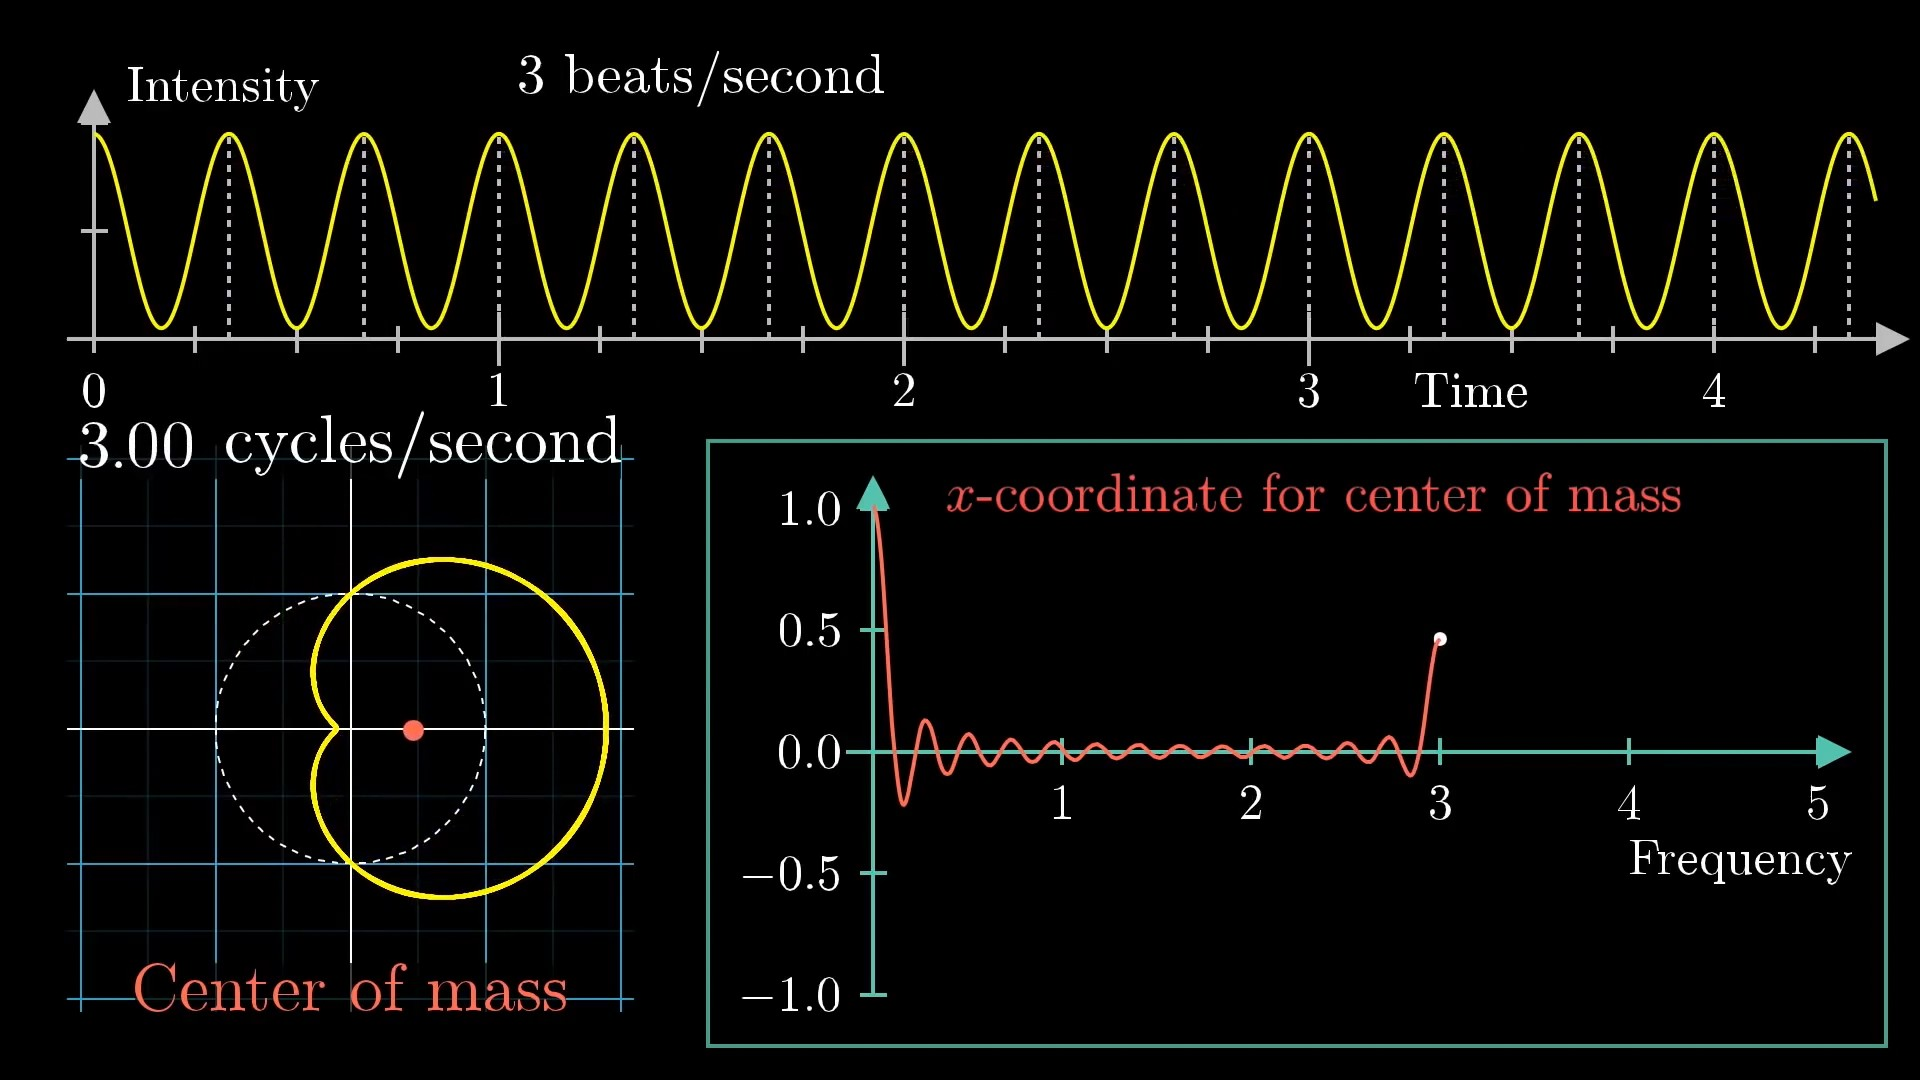
\includegraphics[scale=0.2]{visu_fourier.jpg}
	\caption{Enroulement du signal sur un cercle
	complexe : © 3blue1brown }
\end{figure}



Pour comprendre l'idée général de la Transformé de Fourier, il faut
\textbf{impérativement} regarder cette vidéo : 
\href{https://www.youtube.com/watch?v=spUNpyF58BY}{3blue1brown : But 
what is the Fourier Transform? A visual introduction.}

\underline{Point clefs à retenir}
\begin{itemize}
	\item toutes fonctions périodiques est représentable sur un cercle
		complexe "enroulement d'une fonction". 
	\item En observant le point de gravité (qui sera détaillé dans le
		chapitre \textbf{Fonction holomorphe d'une variable complexe})
		on remarque que lorsque la fréquence
		de représentation sur le cercle coïncide avec celle du signal
		donné alors, la coordonnée $x$ a un comportement spécifique.
		Cette dernière est décentré.
	\item L'objectif de la Transformé de Fourier est de repérer ce
		changement de comportement. Il permet ainsi d'obtenir les
		différentes fréquences que comporte ce signal.
	\item Ainsi le signal et exprimable par les différentes fréquences qu'il
		comportent.
\end{itemize}

Avant de continuer plus loins dans l'analyse de Fourier voici une série de
documents que je recommande particulièrement pour \underline{comprendre la
théorie de Fourier}, mais aussi et surtout, pour \underline{voir l'intérêt
d'étudier Fourier} :
\begin{itemize}
	\item \textbf{3blue1brown} :
		\begin{itemize}
			\item \href{https://www.youtube.com/watch?v=spUNpyF58BY}
				{3blue1brown : But what is the Fourier Transform? 
				A visual introduction.}
			\item \href{https://www.youtube.com/watch?v=r6sGWTCMz2k}{But
				what is a Fourier series? From heat flow to
				circle drawings | DE4}
			\item \href{https://www.youtube.com/watch?v=MBnnXbOM5S4}{The
				more general uncertainty principle, beyond
				quantum} (explique la relation entre la
				transformé de Fourier et le signal (au niveau
				des radars sur Doppler)). Ce qui montre que les
				chauve-souris sont capables instinctivement
				d'effectuer des Transformer de Fourier.
		\end{itemize}
	\item \textbf{Reducible} :
		\begin{itemize}
			\item \href{https://www.youtube.com/watch?v=h7apO7q16V0}{The
				Fast Fourier Transform (FFT): Most Ingenious
				Algorithm Ever?}
		\end{itemize}
	\item \textbf{SmarterEveryDay} :
		\begin{itemize}
			\item \href{https://www.youtube.com/watch?v=ds0cmAV-Yek}{
					What is a Fourier Series? (Explained by
					drawing circles) - Smarter Every Day
					205} redondant à une des vidéos de
					\textbf{3blue1brown} 
			\item \href{https://www.youtube.com/watch?v=4gibcRfp4zA}{
					What is a Fourier Series? (Explained by
					drawing circles) - Smarter Every Day
					205} mathématiques appliqués à l'art
		\end{itemize}
	\item \textbf{Jean-Michel Bony} :
		\begin{itemize}
			\item \underline{Méthodes mathématiques pour les sciences
				physiques}. Dont la structure de ce cours est
				fortement inspirés.
\end{itemize}



\end{itemize}


\chapter{Fonction holomorphe d'une variable complexe}

\end{document}
